\section{Auswertung}
\label{sec:Auswertung}
Jegliche Fehlerrechnung wurde mit der python-Bibliothek uncertainties \cite{uncertainties} absolviert.
Trotz dessen sind die Formeln für die Unsicherheiten in den jeweiligen Abschnitten angegeben.
Allgemeine Rechnungen wurden mit der python-Bibliothek numpy \cite{numpy} automatisiert. 
Die graphischen Unterstützungen wurden mit Hilfe der python-Bibliothek matplotlib \cite{matplotlib} erstellt.
Die Unsicherheiten, welche in den Graphiken eingezeichent sind, sind mit einem Faktor von $0.1$ skaliert worden, da diese sonst durch den
natürlichen Logarithmus zu groß erscheinen würden.
\subsection{Bestimmung der Untergrundrate}
Für die Messung der Untergrundrate wurde ein Zeitintervall von $\symup{\Delta} t = \SI{300}{\second}$ gewählt.
Ingesamt ergaben sieben Messungen die Werte
\begin{equation*}
    N_\text{U} = \{ 129, 143, 144, 136, 139, 126, 158 \} \; \text{.}
\end{equation*}
Der Mittelwert der Untergrundrate beträgt
\begin{equation*}
    \bar{U}_N = 139.2857 \; \text{.}
\end{equation*}
\subsection{Bestimmung der Halbwertszeit von Vanadium}
\label{sub:Vana}
Bevor die Messdaten ausgewertet werden können, muss der Mittelwert der Hintergrundrate mit dem Zeitintervall von $\symup{\Delta} t = \SI{30}{\second}$
abgezogen werden. Dieser beträgt
\begin{equation*}
    \bar{U}_\text{N, \SI{30}{\second}} = 13.9286 \approx 14 \; \text{.}
\end{equation*}
In der Tabelle \ref{tab:vana} sind die Zerfälle der Vanadium-Kerne ohne Abzug der Untergrundrate $\tilde{N}$ und die Zerfälle der Vanadium-Kerne mit Abzug 
der Untergrundrate $N$ aufgetragen.
\begin{table}
    \centering
    \caption{Zerfall der Vanadium-Kerne}
    \label{tab:vana}
    \begin{tabular}{S[table-format=3.0] S[table-format=3.0] S[table-format = 3.2] @{${}\pm{}$} S[table-format = 2.2]
                    S[table-format=4.0] S[table-format=2.0] S[table-format = 2.2] @{${}\pm{}$} S[table-format = 1.2]}
        \toprule
        {$t \mathbin{/} \si{\second}$} & {$\tilde{N}$} & \multicolumn{2}{c} {$N$} & {$t \mathbin{/} \si{\second}$} & {$\tilde{N}$} & \multicolumn{2}{c} {$N$} \\
        \midrule
        30	&    189    & 175.07 & 13.23 & 690  &  35  & 21.07 & 4.59    \\
        60	&    197    & 183.07 & 13.53 & 720  &  19  & 5.07  & 2.25    \\
        90	&    150    & 136.07 & 11.66 & 750  &  28  & 14.07 & 3.75    \\
        120	&    159    & 145.07 & 12.04 & 780  &  27  & 13.07 & 3.62    \\
        150	&    155    & 141.07 & 11.88 & 810  &  36  & 22.07 & 4.70    \\
        180	&    132    & 118.07 & 10.87 & 840  &  25  & 11.07 & 3.33    \\
        210 &	 117    & 103.07 & 10.15 & 870  &  29  & 15.07 & 3.88    \\
        240 &	 107    & 93.07  &  9.65 & 900  &  18  & 4.07  & 2.02    \\
        270 &	 94     & 80.07  &  8.95 & 930  &  17  & 3.07  & 1.75    \\
        300 &	 100    & 86.07  &  9.28 & 960  &  24  & 10.07 & 3.17    \\
        330 &	 79     & 65.07  &  8.07 & 990  &  21  & 7.07  & 2.66    \\
        360 &	  69    & 55.07  &  7.42 & 1020 &  25  & 11.07 & 3.33    \\
        390 &	  81    & 67.07  &  8.19 & 1050 &  21  & 7.07  & 2.66    \\
        420 &	  46    & 32.07  &  5.66 & 1080 &  24  & 10.07 & 3.17    \\
        450 &	  49    & 35.07  &  5.92 & 1110 &  25  & 11.07 & 3.33    \\
        480 &	  61    & 47.07  &  6.86 & 1140 &  17  & 3.07  & 1.75    \\
        510 &	  56    & 42.07  &  6.49 & 1170 &  20  & 6.07  & 2.46    \\
        540 &	  40    & 26.07  &  5.11 & 1200 &  19  & 5.07  & 2.25    \\
        570 &	  45    & 31.07  &  5.57 & 1230 &  20  & 6.07  & 2.46    \\
        600 &	  32    & 18.07  &  4.25 & 1260 &  18  & 4.07  & 2.02    \\
        630 &	  27    & 13.07  &  3.62 & 1290 &  16  & 2.07  & 1.44    \\
        660 &	  43    & 29.07  &  5.39 & 1320 &  17  & 3.07  & 1.75    \\
    \bottomrule     
    \end{tabular}
\end{table}
Zu der Bestimmung der Halbwertszeit wird die Beziehung \eqref{eqn:penis} logarithmiert, so dass sich die Form
\begin{equation}
\ln \left (N \right ) = \ln \left (N_0 \left (1-\symup{e}^{\SI{-30}{\second} \lambda} \right ) \right )   - \lambda t 
\end{equation}
ergibt.
Somit lässt sich eine lineare Ausgleichsrechung mit der Geradengleichung
\begin{equation}
    y = at + b 
\end{equation}
durchführen. 
Für die Regressionsparameter $a$ und $b$ ergibt sich
\begin{align*}
    a &= \SI{-0.0032(2)}{\per\second} = - \lambda\\
    b &= \num{5.1865(1275)} \; \text{.}
\end{align*}
\noindent Mit Hilfe der Gleichung \eqref{eqn:halbw} lässt sich die Halbwertszeit zu
\begin{figure}
    \centering
    \caption{Zerfallskurve von Vanadium}
    \label{fig:vana}
    \includegraphics{build/vana.pdf}
\end{figure}
\begin{equation*}
\tau = \SI{219(11)}{\second}
\end{equation*}
bestimmen.
\FloatBarrier
\subsection{Bestimmung der Halbwertszeit von Rhodium}
Wie bereits in Abschnitt \ref{sub:Vana} muss der Mittelwert der Hintergrundrate abgezogen werden.
Da die übrigen Rhodium-Kerne mit einem Intervall von $\symup{\Delta} t = \SI{15}{\second}$ gemessen wurden, muss der Mittelwert der Untergrundrate
auf dieses Zeitintervall herunterskaliert werden.
\begin{equation*}
    \bar{U}_\text{N, \SI{15}{\second}} = 6.9644 \approx 7 \; \text{.}
\end{equation*}
In der Tabelle \ref{tab:vana} sind die Zerfälle der Rhodium-Kerne ohne Abzug der Untergrundrate $\tilde{N}$ und die Zerfälle mit Abzug 
der Untergrundrate $N$ aufgetragen.
\begin{table}
    \centering
    \caption{Gemessene Rhodium-Zerfälle}
    \label{tab:rho}
    \begin{tabular}{S[table-format=3.0] S[table-format=3.0] S[table-format = 3.2] @{${}\pm{}$} S[table-format = 2.2]
                    S[table-format=3.0] S[table-format=2.0] S[table-format = 2.2] @{${}\pm{}$} S[table-format = 1.2]}
        \toprule
        {$t \mathbin{/} \si{\second}$} & {$\tilde{N}$} & \multicolumn{2}{c} {$N$} & {$t \mathbin{/} \si{\second}$} & {$\tilde{N}$} & \multicolumn{2}{c} {$N$} \\
        \midrule
        15  &  667 & 660.04 & 25.69 & 345 & 36 & 29.04 & 5.39 \\
        30  &  585 & 578.04 & 24.04 & 360 & 38 & 31.04 & 5.57 \\
        45  &  474 & 467.04 & 21.61 & 375 & 34 & 27.04 & 5.20 \\
        60  &  399 & 392.04 & 19.80 & 390 & 40 & 33.04 & 5.74 \\
        75  &  304 & 297.04 & 17.23 & 405 & 21 & 14.04 & 3.74 \\
        90  &  253 & 246.04 & 15.68 & 420 & 35 & 28.04 & 5.29 \\
        105 &  213 & 206.04 & 14.35 & 435 & 33 & 26.04 & 5.10 \\
        120 &  173 & 166.04 & 12.88 & 450 & 36 & 29.04 & 5.39 \\
        135 &  152 & 145.04 & 12.04 & 465 & 20 & 13.04 & 3.61 \\
        150 &  126 & 119.04 & 10.91 & 480 & 24 & 17.04 & 4.12 \\
        165 &  111 & 104.04 & 10.20 & 495 & 30 & 23.04 & 4.80 \\
        180 &   92 & 85.04  & 9.22  & 510 & 30 & 23.04 & 4.80 \\
        195 &   79 & 72.04  & 8.49  & 525 & 26 & 19.04 & 4.36 \\
        210 &   74 & 67.04  & 8.19  & 540 & 28 & 21.04 & 4.58 \\
        225 &   60 & 53.04  & 7.28  & 555 & 23 & 16.04 & 4.00 \\
        240 &   52 & 45.04  & 6.71  & 570 & 20 & 13.04 & 3.61 \\
        255 &   56 & 49.04  & 7.00  & 585 & 28 & 21.04 & 4.58 \\
        270 &   53 & 46.04  & 6.78  & 600 & 17 & 10.04 & 3.16 \\
        285 &   41 & 34.04  & 5.83  & 615 & 26 & 19.04 & 4.36 \\
        300 &   36 & 29.04  & 5.39  & 630 & 19 & 12.04 & 3.46 \\
        315 &   37 & 30.04  & 5.48  & 645 & 13 & 6.04  & 2.45 \\
        330 &   32 & 25.04  & 5.00  & 660 & 17 & 10.04 & 3.16 \\
        \bottomrule     
    \end{tabular}
\end{table}
\begin{figure}
    \centering
    \caption{Zerfallskurve von Rhodium}
    \label{fig:rho}
    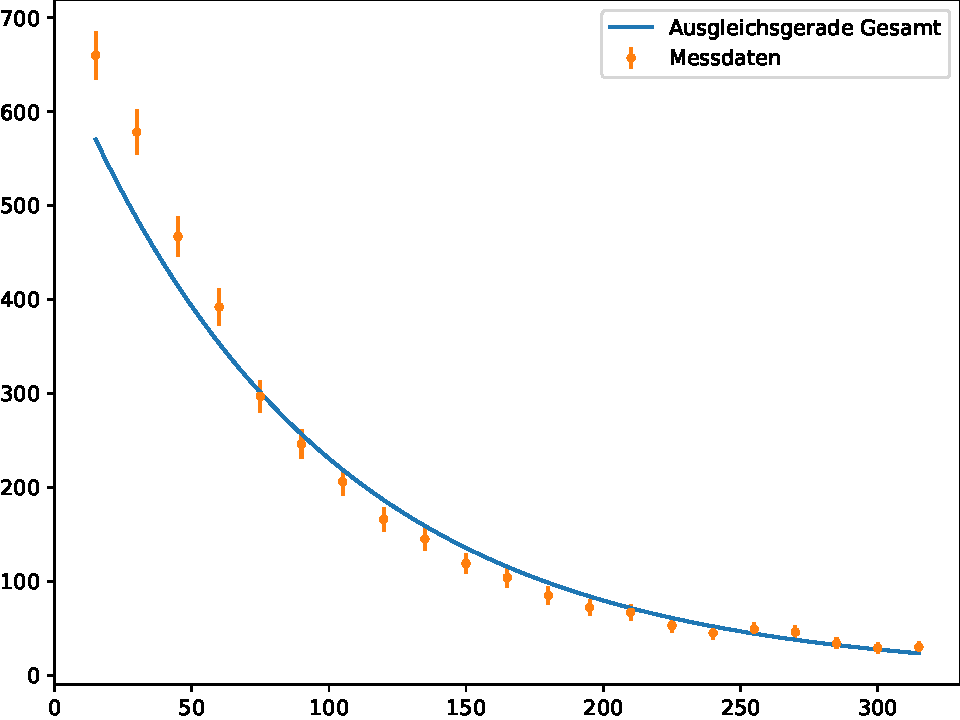
\includegraphics{build/rho.pdf}
\end{figure}
In der Abbildung \ref{fig:rho} sind die Ausgleichsgeraden für den kurzlebigen Zerfall und für den gesamten Zerfall für die Zeiten $t < t^*$ eingezeichnet.
Um die einzelnen Geraden zu ermitteln, ist es von Nöten den Zeitpunkt $t^*$ zu bestimmen.
Dieser kann der Abbildung \ref{fig:rho} graphisch entnommen werden.
Dort ist zu erkennen, dass der langlebige Prozess ab $t^* = \SI{300}{\second}$ einsetzt.
Für die Gerade aller Messdaten für $t < t^*$
\begin{equation}
    y_g = a_g t_g + b_g
\end{equation}
ergeben sich die Parameter zu 
\begin{align*}
    a_g &= \SI{-0.0123(2)}{\per\second} \\
    b_g &= \num{6.6881(2698)} \; \text{.}
\end{align*}
Die Parameter der Ausgleichgerade ab $t^*$
\begin{equation}
    y_l = a_l t + b_l
\end{equation}
ergeben sich zu
\begin{align*}
    a_l &= \SI{-0.0030(5)}{\per\second} = - \lambda_l \\
    b_l &= \num{4.4212(2608)} \; \text{.}
\end{align*}
Daraus kann man die Halbwertszeit von \ce{ ^{104\text{i}}_45 Rh} zu 
\begin{equation*}
    \tau_l = \SI{230(40)}{\second}
\end{equation*}
bestimmen.
Um die Werte des kurzlebigen Zerfalls zu errechnen, werden von den gesamten Werten für $t < t^*$ die errechneten Werte des langlebigen Zerfalls abgezogen,
so dass eine erneute Ausgleichsrechung durchgeführt werden kann.
Die Parameter der Ausgleichgerade des kurzlebigen Zerfalls
\begin{equation}
    y_k = a_k t + b_k
\end{equation}
ergeben sich zu
\begin{align*}
    a_k &= \SI{-0.0169(4)}{\per\second} = - \lambda_k \\
    b_k &= \num{6.7234(481)} \; \text{.}
\end{align*}
Daraus kann die Halbwertszeit von \ce{ ^104_45 Rh} zu 
\begin{equation*}
    \tau_l = \SI{41.0(11)}{\second}
\end{equation*}
bestimmt werden.
In der Tabelle \ref{tab:rhokurz} und \ref{tab:rholang} sind die errechneten kurz- und langlebigen Zerfälle gelistet.
\begin{figure}
    \centering
    \caption{Kurz- und langlebige Ausgleichgerade des Rhodium-Zerfalls}
    \label{fig:rhoaang}
    \includegraphics{build/rho2.pdf}
\end{figure}
\begin{table}
    \centering
    \caption{Errechnete kurzlebige Rhodium-Zerfälle}
    \label{tab:rhokurz}
    \begin{tabular}{S[table-format=3.0]  S[table-format = 3.2] @{${}\pm{}$} S[table-format = 2.2]}
        \toprule
        {$t \mathbin{/} \si{\second}$} & \multicolumn{2}{c} {$N_k$}  \\
        \midrule
         15 & 645.30 & 25.40 \\
         30 & 500.72 & 22.38 \\
         45 & 388.54 & 19.71 \\
         60 & 301.49 & 17.36 \\  
         75 & 233.94 & 15.30 \\  
         90 & 181.53 & 13.47 \\  
        105 & 140.86 & 11.87 \\  
        120 & 109.30 & 10.45 \\  
        135 &  84.81 & 9.21  \\ 
        150 &  65.81 & 8.11  \\  
        165 &  51.06 & 7.15  \\  
        180 &  39.62 & 6.29  \\  
        195 &  30.75 & 5.54  \\ 
        210 &  23.86 & 4.88  \\ 
        225 &  18.51 & 4.30  \\ 
        240 &  14.36 & 3.79  \\ 
        255 &  11.15 & 3.34  \\ 
        270 &   8.65 & 2.94  \\ 
        285 &   6.71 & 2.59  \\ 
        \bottomrule     
    \end{tabular}
\end{table}
\begin{table}
    \centering
    \caption{Errechnete langlebige Rhodium-Zerfälle}
    \label{tab:rholang}
    \begin{tabular}{S[table-format=3.0]  S[table-format = 3.2] @{${}\pm{}$} S[table-format = 2.2]}
        \toprule
         {$t \mathbin{/} \si{\second}$} & \multicolumn{2}{c} {$N_l$} \\
        \midrule
        300 &  33.46 & 5.78\\
        315 &  31.97 & 5.65\\
        330 &  30.55 & 5.53\\
        345 & 29.19 & 5.40 \\  
        360 & 27.89 & 5.28 \\  
        375 & 26.65 & 5.16 \\  
        390 & 25.46 & 5.05 \\  
        405 & 24.33 & 4.93 \\  
        420 & 23.24 & 4.82 \\ 
        435 & 22.21 & 4.71 \\  
        450 & 21.22 & 4.61 \\  
        465 & 20.27 & 4.50 \\  
        480 & 19.37 & 4.40 \\ 
        495 & 18.51 & 4.30 \\ 
        510 & 17.69 & 4.21 \\ 
        525 & 16.90 & 4.11 \\ 
        540 & 16.15 & 4.02 \\ 
        555 & 15.43 & 3.93 \\ 
        570 & 14.74 & 3.84 \\ 
        585 & 14.08 & 3.75 \\ 
        600 & 13.46 & 3.67 \\ 
        615 & 12.86 & 3.59 \\ 
        630 & 12.28 & 3.50 \\ 
        645 & 11.74 & 3.43 \\ 
        660 & 11.22 & 3.35 \\ 
        \bottomrule     
    \end{tabular}
\end{table}
Der Fehler der Zerfälle lässt sich mittels
\begin{equation}
    \symup{\Delta} N = \sqrt{\tilde{N} - N_U} 
\end{equation}
errechnen.
Nach der Gaußschen Fehlerfortpflanzung wird die Unsicherheit der Halbwertszeit durch
\begin{equation}
    \symup{\Delta} \tau = \frac{\ln \left (2 \right )}{\lambda^2} \symup{\Delta} \lambda
\end{equation}
errechnet.